El propósito de todo sitio web es ser utilizado y aprovechado por la mayor cantidad de personas posibles, y es por eso que el punto clave del desarrollo web se encuentra en cómo los desarrolladores proporcionan un sitio web que cumpla con ese propósito. Para conseguir dicho propósito se deben tener múltiples consideraciones que abarca desde la experiencia de usuario hasta la calidad de la infraestructura y el código realizado. Cuando hablamos de experiencia de usuario nos referimos al resultado de la interacción del usuario con los distintos elementos que posee el sitio web, de tal forma que el usuario pueda tener una experiencia positiva al hacer uso de dichos elementos. Petter Morville \cite{UXFactors} propone que para lograr una buena experiencia de usuario se debe tener en cuenta el correcto uso de los siguientes factores: 

\begin{itemize}
    \item Utilidad: el producto realizado debe ser de utilidad para el público objetivo.
    \item Usabilidad: debe ser un sistema que sea simple y fácil de usar para el usuario.
    \item Deseabilidad: cuando un producto es deseable, los usuarios se sienten atraídos a el.
    \item Encontrable: se debe construir un sistema que sea navegable y fácil de encontrar, de tal forma que los usuarios puedan encontrar lo que necesiten fácilmente.
    \item Accesibilidad: el sistema debe poder ser usado por la mayor cantidad de personas posibles.
    \item Credibilidad: el sistema debe proporcionar seguridad al usuario acerca de la credibilidad de su contenido
    \item Valor: una experiencia de usuario valiosa implica un buen uso de los demás factores.
\end{itemize}

Sin embargo, para que sea posible cumplir con todos los factores que permiten una buena experiencia de usuario,
es indispensable realizar un código de calidad que proporcione al sitio web un buen rendimiento, permitiendo al sitio web
desempeñar su función correctamente.

En este capítulo presentaremos las herramientas que nos facilitaran el trabajo para lidiar con las problemáticas mencionadas.

\section{Arquitectura}

Para que una aplicación sea descubierta y usada por internautas es fundamental que tenga una buena relación con los motores de búsqueda.

Sin embargo también para asegurar la larga vida y mantenibilidad de la aplicación y la facilidad de desarrollo se debe tomar en cuenta herramientas extensamente empleadas contemporáneamente como Angular, React y Vue.

El problema entonces recae en que estas tecnologías son meramente para SPA. Lo que implica entonces que no existe una noción "real" de seo - En las SPA el enrutamiento ocurre del lado del cliente usando javascript, y en consecuencia los crawlers de los motores de búsqueda no saben interpretar estas paginas.

Como remedio surge un nuevo paradigma, que es el que vamos a usar para esta aplicación, conocido como Server Side Rendering; donde se utiliza estas tecnologías SPA como un motor de plantillas para retornar un HTML que los motores de búsqueda puedan entender, y después por un proceso conocido como hydration, las aplicaciones en el lado del cliente dejan de comportarse como HTML plano y retoman sus funcionalidades de SPA.

Asi entonces llegamos al perfecto balance en el que tenemos herramientas actuales y fáciles de usar, que también cumplen con los requerimientos de los motores de búsqueda para indexar nuestras paginas.


\section{Tecnologías para el desarrollo}

Actualmente existe un catalogo muy amplio de tecnologías de desarrollo web, por lo que escoger las debidas herramientas y sobre todo analizar las compatibilidades entre estas herramientas pueden ser el punto clave para obtener la mejor eficiencia y experiencia de usuario.

Para nuestro proyecto haremos uso de un servidor cuyo propósito será obtener los datos y transformarlos de forma que el cliente los pueda usar directamente sin necesidad usar mucho computo, esto con el propósito de proporcionar una mejor experiencia de usuario.

El este capitulo hablaremos de las herramientas de desarrollo web usadas para llevar a cabo el proyecto, y las descompondremos en 2 categorías: Servidor y Cliente.

\section{Servidor}

\subsection{MongoDB}

MongoDB es un sistema de base de datos NoSQL, orientado a documentos y de código abierto. En lugar de guardar los datos en tablas, tal y como se hace en las bases de datos relacionales, MongoDB guarda estructuras de datos BSON (una especificación similar a JSON) con un esquema dinámico, haciendo que la integración de los datos en ciertas aplicaciones sea más fácil y rápida.

\iffalse
    \begin{figure}
        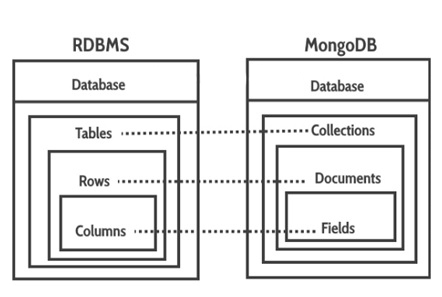
\includegraphics[scale=1.2]{mongodb-structure.jpg}
        \caption{Comparación de estructura de datos entre MongoDB y los RDBMS (sistema de gestión de bases de datos relacionales)}
    \end{figure}
\fi

\subsection{Fastify}

Fastify es un framework web para Node.js de código abierto concentrado en proporcionar el mejor rendimiento, y una arquitectura flexible. \\

Si comparamos la velocidad de Fastify con otros frameworks web como Express, tal como podemos ver en la figura \ref{fig:fastify_vs_express}, notamos que Fastify es aproximadamente un 20\% más rápido que Express. \\

\begin{figure}
    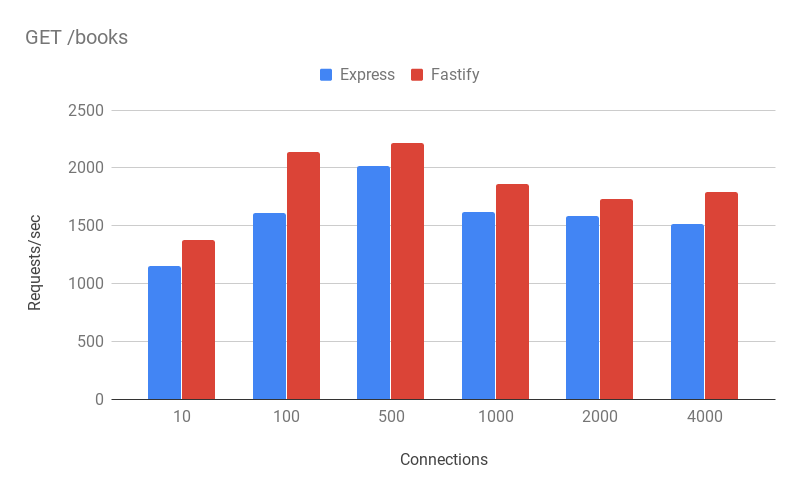
\includegraphics[scale=0.5]{fastify_vs_express.png}
    \caption{ Número de peticiones por segundo para distinta cantidad de conexiones}
    \label{fig:fastify_vs_express}
\end{figure}


\section{Cliente}

Para la realización de este proyecto se usarán las siguientes tecnologías:

\subsection{ReactJS}

ReactJS es una librería de JavaScript de código abierto desarrollada por Facebook para facilitar la creación de componentes interactivos, reutilizables, para desarrollos de interfaces de usuario, especialmente aplicaciones de una sola página.\\

React maneja el concepto de \say{programación reactiva} haciendo uso de un DOM Virtual, lo le permite determinar qué partes del DOM han cambiado comparando contenidos entre la versión nueva y la almacenada den el DOM virtual, para así propagar los datos generando cambios en la aplicación, es decir, los datos \say {reaccionan} ejecutando una serie de eventos.\\

Este concepto de reactividad es lo que hace a la librería altamente eficiente, ya que limita la actualización del DOM solamente a los elementos que han cambiado.\\

Otras características que destacan en React son:\\

\begin{itemize}
    \item \textbf{Componentes} \hfill \\

          El código de React es hecho con entidades llamadas componentes. Los componentes pueden ser renderizados en elementos particulares del DOM usando la librería de React DOM. Estos componentes son capaces de recibir parámetros conocidos como "propiedades del componente" de la siguiente forma: \hfill \\

          \begin{lstlisting}
                ReactDOM.render(<Greeter greeting="Hello World!" />, document.getElementById('myReactApp'));
            \end{lstlisting}

          Las 2 formas de declarar componentes en react es mediante el uso de funciones o clases, y generalmente se usa una de las dos opciones de forma situacional.

    \item \textbf{JSX} \hfill \\

          JSX, también llamado Javascript XML, es una extension a la sintaxis del lenguaje javascript. Este provee una forma de estructurar componentes usando una sintaxis familiar para muchos desarrolladores. Los componentes de React son usualmente escritos usando JSX, aunque también pueden ser escritos usando Javascript puro.

          Un ejemplo de código JSX:

          \begin{lstlisting}
                class App extends React.Component {
                    render() {
                        return (
                        <div>
                            <p>Header</p>
                            <p>Content</p>
                            <p>Footer</p>
                        </div>
                        );
                    }
                }
            \end{lstlisting}

    \item \textbf{Hooks} \hfill \\

          Los hooks son funciones que permiten a los desarrolladores \say{engancharse} a los estados de React y a ciertos puntos dentro del ciclo de vida de los componentes.

          React proporciona algunos hooks integrados tales como: useState, useContext, useReducer, useMemo y useEffect, los cuales son los mas usados y permiten controlar los estados y eventos respectivamente.


\end{itemize}

\subsection{Next.js}

Next.js es un framework desarrollado encima de Node.js que permite a las aplicaciones de React usar funcionalidades como el renderizado del lado servidor y la generación de paginas web estáticas.\\

Por defecto, Next.js pre-renderiza cada pagina. Esto significa que Next.js genera HTML para cada pagina en adelanto, en vez de hacerse con Javascript del lado del cliente. Pre-renderizado puede resultar en mejor rendimiento y SEO.\\

Cada HTML generado es asociado con el mínimo código Javascript necesario para que funcione la pagina. Cuando una página es cargada en el explorador, su código javascript se ejecuta y hace la página totalmente interactiva. A este proceso de le conoce como \say{hydration}

Next.js ofrece 2 formas de pre-renderizado:

\begin{itemize}
    \item Generación estática: El HTML es generado a tiempo de ejecución y será reutilizado en cada petición.
    \item Renderizado lado servidor: El HTML es generado en cada petición
\end{itemize}

\subsection{Material UI}

Material UI es un framework de React que sigue los principios de Material Design \ref*{MaterialDesignPrinciples}, el cual fue creado por Google. Su objetivo es facilitar la creación de interfaces gráficas con el uso de componentes de React que ya fueron probados y aseguran una buena experiencia de usuario. Material UI se destaca ante otros frameworks UI por ser uno de los que posee mayor mantenibilidad (mayor cantidad de contribuyentes) y una gran variedad de componentes.

Material UI también posee la posibilidad de crear temas, lo que permite modificar los estilos de los componentes predeterminados de la librería de forma global en caso de necesitarse un diseño más personalizado.

A continuación se monstrará el uso de algunos componentes que ofrece la libreria:

\begin{itemize}
    \item Botones\\

          \begin{lstlisting}
                <Button variant="text">Text</Button>
                <Button variant="contained">Contained</Button>
                <Button variant="outlined">Outlined</Button>
            \end{lstlisting}

          donde el parametro variant representa una variante visual del boton, las cuales son usadas dependiendo del proposito/importancia del botón.

    \item Selectores\\

          \begin{lstlisting}
                <FormControl fullWidth>
                    <InputLabel id="demo-simple-select-label">Age</InputLabel>
                    <Select
                    labelId="demo-simple-select-label"
                    id="demo-simple-select"
                    value={age}
                    label="Age"
                    onChange={handleChange}
                    >
                        <MenuItem value={10}>Ten</MenuItem>
                        <MenuItem value={20}>Twenty</MenuItem>
                        <MenuItem value={30}>Thirty</MenuItem>
                    </Select>
                </FormControl>
            \end{lstlisting}

          El componente selector debe estar dentro de un componente de FormControl para que sea posible obtener sus datos al momento de enviar el formulario.

    \item Sliders\\

          \begin{lstlisting}
                <Slider aria-label="Volume" value={25} onChange={handleChange} />
            \end{lstlisting}

          Donde su parametro value es el valor por default del slider y el parámetro onChange recibe una funcion que se ejecuta al mover el slider.

\end{itemize}

